\section{Person Recognition}

An Operator is introduced to the robot, which needs to learn what the Operator looks like. Once the robot has gathered enough information about the Operator, the Operator mixes within a crowd and the robot needs to find the Operator. Once the robot has found its Operator, it must state some information about the Operator and the crowd, such as genders.

\subsection{Goal}
The robot has to identify the Operator within a crowd and state information about the Operator and the crowd.

\subsection{Focus}

This test focuses on people detection and recognition; as well as pose recognition and human-robot interaction with unknown people.

\subsection{Setup}

\begin{enumerate}
\item \textbf{Operator:} A \quotes{professional} operator is selected by the TC to test the robot. 
  This person may a different be drafted from the crowd in each run.
\item \textbf{Other people} There are no restrictions on other people walking by or standing around throughout the complete task.
\end{enumerate}

\subsection{Task}
\paragraph{This test may also be held outside the arena
  This is in order to have the possibility to run multiple robots in parallel and reduce the total time needed to test all robots.}

\begin{enumerate}

  \item \textbf{Start:} The robot starts at a designated starting position, and waits for the \quotes{professional} operator.

  \item \textbf{Memorizing the operator:} The robot has to memorize the operator.   During this phase, the robot may instruct the operator to follow a certain setup procedure.

  \item \textbf{Learning operator name:} Optionally, the robot may ask the operator for his/her name and make the interaction after finding the operator again more natural.

  \item \textbf{Waiting 10 seconds:} Once the robot states it has finished memorizing the operator, it must wait 10 seconds while the operator walks around and mixes with the crowd.

  \item \textbf{Find the crowd:} After the time elapses, the robot must turn around about $180\degree$, find the crowd, and start looking for the operator.
  \begin{itemize}

    \item \textbf{Crowd size:} The crowd may contain between 5 and 10 people, standing or sitting or lying within an  area of 5 meters (diameter).

    \item \textbf{Crowd position:} The crowd will be located behind the robot at a distance between 2 and 3 meters apart.
  \end{itemize}

  \item \textbf{Finding the operator:} Once the crowd has been located, the robot must greet the operator (optionally by name) and state their gender, pose (sitting, standing, raised arm), and relative position within the crowd.   Alternatively to state the relative position of the operator, the robot may point or approach to the operator. In any case, it must be clear to the referees that the robot has found the operator, unambiguously. Examples include:
  \begin{itemize}

    \item My operator is the girl sitting left most of the crowd.

    \item Mary, you are standing behind the bearded man with black shirt wearing glasses.

    \item Adam is the blond guy standing in the center between two female people.
  \end{itemize}

  \textbf{Remark:} In the case of the slightest ambiguity, no points will be granted.This includes the referees not being able to understand or hear the robot.

  \item \textbf{Describing the crowd}: Finally, robot must tell the size of the crowd and how many men, women and unidentified people are (even including children).

  \item \textbf{Delivering report file}: Immediately after the test, an USB pen-drive will be collected by the referees from the robot. The pen-drive must contain a report file as described further.
\end{enumerate}

\subsection{Report file:}
Robots must create a PDF report file stored in a USB-stick attached to the robot to be given to the TC after the test, which will be used for scoring. The report must be as follows:
\begin{itemize}

  \item \textbf{File name:} The name of the file must be: \texttt{TeamName-Try-Timestamp.pdf}

  \item \textbf{Team name:} The report file \textbf{must contain the name of the team}.

  \item \textbf{Operator's picture: } The report file must include a picture of the operator with a caption stating operator's gender and, if given, the operator's name. Drawing a frame enclosing the region(s) used for recognition is advised.

  \item \textbf{Crowd's picture:} Under the operators information, the report file must include a picture of the crowd with a labeled frame enclosing each detected person, and a set of captions stating their genders and, in the case of the operator, the pose. 
\end{itemize}

\begin{figure}[tbp]
  \centering
  \subfloat[Operator]{\label{fig:person_recognition_operator}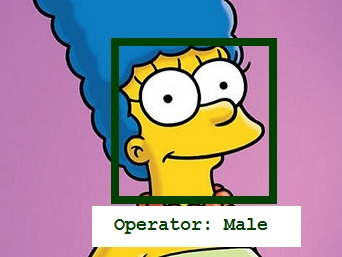
\includegraphics[height=46mm]{images/person_recognition_operator.jpg}} ~ 
  \subfloat[Crowd]{\label{fig:person_recognition_crowd}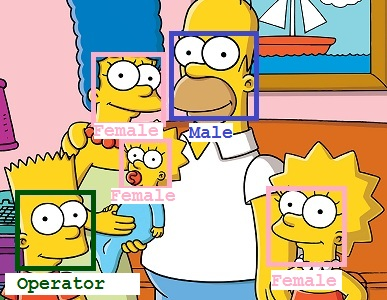
\includegraphics[height=46mm]{images/person_recognition_crowd.jpg}}
  \caption{Report picture examples: The operator's gender was incorrectly labeled and wasn't found in the crowd, however four out of four genders are specified correctly. No pose is stated.}
  \label{fig:person_recognition}
\end{figure}

\subsection{Additional rules and remarks}
\begin{enumerate}
\item \textbf{Waiting \& Continue Rule:} Instead of waiting 10 seconds the robot may wait for a spoken command. Since this test is not concerned with audio and speech recognition, therefore there is no penalty when using the Continue Rule (see Section \refsec{rule:asrcontinue}). A single key press used as start command is also allowed.
\item \textbf{Disturbances from outside:} If a person from the audience (severely) interferes with the robot in a way that makes it impossible to solve the task, the team may repeat the test immediately.
\item \textbf{Children:} Note that the operator and crowd may be members of the audience as well, which may include children. A robot only looking up may look over a child operator. 
\item \textbf{Preparation:} The robot needs to wait for about 1 min before the operator appears in front of the robot. During this waiting time the team is not allowed to touch the robot.
\item \textbf{Instructing the operator:} The robot interacts with the operator, not the team. The team is not allowed to instruct the operator.
\end{enumerate}

\subsection{Data recording}
  Please record the following data (See \refsec{rule:datarecording}):
  \begin{itemize}
   \item Images These will not be publicly available due to privacy concerns of the operator and crowd. 
  \end{itemize}


%\subsubsection{Referee instructions}
%
%The referee needs to
%\begin{itemize}
%\item 
%\item 
%\end{itemize}

\subsection{OC instructions}

\textbf{2 hours before the test}
\begin{itemize}
\item Select the \quotes{professional} operator(s).
\item Select the crowd.
\end{itemize}

\textbf{During the test}
\begin{itemize}
\item Check safe operation of the robot; the robot needs to be stopped immediately if a person is going to be touched by the robot
\end{itemize}

\newpage
\subsection{Score sheet}
The maximum time for this test is 5 minutes.

\begin{tabularx}{\textwidth}{X r c c c }

	\textbf{Action} & \textbf{Score} & \textbf{$1^{st}$ try} & \textbf{$2^{nd}$ try} & \textbf{$3^{rd}$ try} \\ \hline
	& & & & \\ 
	\textit{\textbf{Operator}} \\
	Approach or point at the operator & $30$ & \hrulefill & \hrulefill & \hrulefill \\
	Correctly state operator's gender & $30$ & \hrulefill & \hrulefill & \hrulefill \\
	Correctly state operator's pose & $30$ & \hrulefill & \hrulefill & \hrulefill \\
	& & & & \\ 
	\textit{\textbf{Crowd}} \\
	Correctly state crowd's size & $20$ & \hrulefill & \hrulefill & \hrulefill \\
	Correctly state crowd's number of men & $20$ & \hrulefill & \hrulefill & \hrulefill \\
	Correctly state crowd's number of women & $20$ & \hrulefill & \hrulefill & \hrulefill \\ \hline
	& & & & \\ 
	\textit{\textbf{Score per try}} & $150$ & \hrulefill & \hrulefill & \hrulefill \\ 
	& & & & \\ 
	\textbf{Total Score} & $150$ & & & \\ \cline{3-5}

\end{tabularx}\\


% Local Variables:
% TeX-master: "Rulebook"
% End:


% Local Variables:
% TeX-master: "Rulebook"
% End:
